\chapter{SM-02}
\begin{align*}
\text{Boltzman entrophy relation: }&S=K \ln \Omega\\
\text{striling approximation: }\ln n !&=n \ln n-n\\
\text{Number of microstates: }
\Omega_{M B}&=\underset{i}{\pi}\left(g_{i}\right)^{n_{i}}\\
\Omega_{B E}&=\underset{i}{\pi}\frac{\left(n_{i}+g_{i}-1\right) !}{n_{i} !(g i-1) !}\\
{ }^{\Omega_{F D}}&=\underset{i}{\pi}{g i }\  C_{n_{i}}\\
g_{i} &\rightarrow\text{ degeneracy}\\
n_{i} &\rightarrow\text{ identical Particles}\\
\text{Energy distribution function :}f(E)&=\frac{n_{i}}{g_{i}}
\end{align*}
Q.The number of ways in which $N$ identical bosons can distributed in two energy levels is 
 \begin{tasks}(4)
	\task[\textbf{a.}] $N+1$
	\task[\textbf{b.}]$N(N-1) \mid 2$
	\task[\textbf{c.}]$N(N+1) \mid 2$
	\task[\textbf{d.}]$N$ 
\end{tasks}
\begin{answer}
	\begin{align*}
	\Omega&=N_ {C_n}=\frac{N !}{n !(N-n) !}\hspace{2cm}\underset{\text{-------------- }e}{n}\\
	\text { entropy }(s)&=k \ln \Omega=k \ln \frac{N !}{n !(N-n) !}\hspace{1.1cm}\underset{\text{-------------- } 0}{(N-n)}\\
	\operatorname{s\alpha } &\ln \frac{N !}{n !(N-n) !}
	\end{align*}
		So the correct answer is \textbf{Option (d)}
\end{answer}
\begin{note}
	Probability will be maximum for equal distribution.
\end{note}
Q. Let $N_{M B}, N_{B E}, N_{F D}$ denote the number of ways in which two particles can be distributed in two energy states according to maxwell-Boltzmann, Bose-Einstein \& fermi-Dirac statistics respectively. Then $N_{M B}: N_{B E}: N_{F D}$ is:
 \begin{tasks}(4)
	\task[\textbf{a.}]$4: 3: 1$
	\task[\textbf{b.}] $4: 2: 3$
	\task[\textbf{c.}]$4: 3: 3$
	\task[\textbf{d.}] $4: 3: 2$
\end{tasks}
\begin{answer}
	\begin{align*}
	\Omega_{M B}&=\left(g_{i}\right)^{n_{i}}=(2)^{2} \Rightarrow 4 \\
	\Omega_{B E}&=\frac{\left(n_{i}+g_{i}-1\right) !}{n_{i} !((-i-1) !}=\frac{(2+2-1) !}{2 !(2-1) !}=\frac{3 !}{2 !}=3\\
	\Omega_{F D}&=g i C_{n_{i}}=\frac{2 !}{2 ! 1 !}=1\\
	&4:3:1
	\end{align*}
	So the correct answer is \textbf{Option (a)}
\end{answer}
\textbf{Relative Probability: }\\
\begin{align*}
r&=\frac{P_1}{P_2}=\frac{\text{Probability of finding particle in same state}}{\text{Probability of finding particle in different state.}}\\
r_{B E}:& r_{M B}: r_{F \cdot D}=1: 1 / 2: 0\\
\Rightarrow& U_{B E} \leqslant U_{M B} \leqslant U_{F D} \Rightarrow P_{B E} \leqslant P_{M B} \leqslant P_{F D} \\\\
\end{align*}

Q If $N$ particle are to be distributed into two groups such that group i contain $n_1$ particles and group two contains $n_2$ particles, and $N=n_1+n_2$ Find the number of ways of distribution?
\begin{answer}
	\begin{align*}
	\Omega&={ }^{N} C_{n_{1}} \text { or }{ }^{N} C_{n_{2}} 4 N=n_{1}+n_{2}\\
	N_{C_{n_{i}}}&=\frac{N !}{n_{1} !(N-n) !}=\frac{N !}{n_{1} ! n_{2} !}\\
	&\text{similaarly, for $ni$ particles}\\
	\Omega&=\frac{N!}{n_1!n_2!.......n_i!}
	\end{align*}
\end{answer}
Q. A system has energy levels $E_{0}, 2 E_{0}, 3 E_{0}, \ldots .$ where the excited states are triphy generate four non-interacting bosons are placed in this system. If the total energy og these bosons is $5E_0$ the number of microstates is:
 \begin{tasks}(4)
	\task[\textbf{a.}]2
	\task[\textbf{b.}]3
	\task[\textbf{c.}]4
	\task[\textbf{d.}] 5
\end{tasks}
\begin{answer}
	\begin{figure}[H]
		\centering
		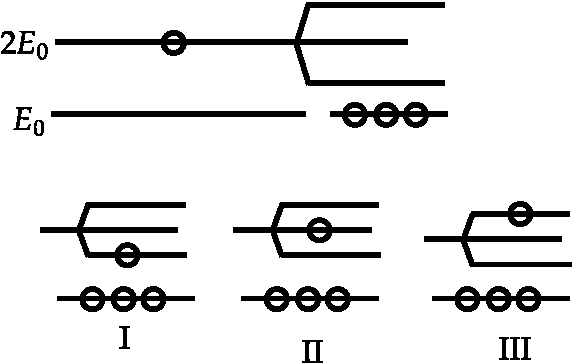
\includegraphics[height=4cm,width=6cm]{SP-12}
	\end{figure}
	So the correct answer is \textbf{Option (b)}
\end{answer}
\textbf{Phase Space}:(Position + momentum) space\\
volume of single phase cell: $d \tau=h^{f} \quad f \rightarrow D O F$\\
allowed vol. of phace space: $\int d^{3} q \int d^{3} p$\\
$$
V_{p} \Rightarrow V \times \frac{4}{3} \pi p^{3}\text{( for 3-Dim).}
$$
\textbf{Non-Relativistic Free Particle: }$E=p^2/2m$\\
\renewcommand*{\arraystretch}{2}
 \begin{tabular}{|p{4cm}|p{4cm}|p{4cm}|}
 	\hline
 3-Dimensional&2-Dimensional&1-Dimensional\\\hline
 $d \tau=h^{3}$&$d \tau=h^{2}$&$d \tau=h$\\\hline
 $V_{p}=V \times \frac{4}{3} \pi p^{3}$&$V_{p}=A \times \pi p^{2}$&$V_p=L\times2p$\\\hline
 $\Omega=\frac{V \cdot \frac{4}{3} \pi p^{3}}{\hbar^{3}}$&$\Omega(p)=\frac{\pi \times \pi p^{2}}{h^{2}}$&$\Omega(p)=\frac{L \times 2 p}{h}$\\\hline
 $\Omega(E)=\frac{\mu\pi V(2mE)^3}{3h^3}$&$\Omega(E)=\frac{\pi A(2mE)}{h^2}$&$\Omega(E)=\frac{2L\sqrt{2mE}}{h}$\\\hline
 $\Omega^{\prime}(E)=\frac{2 \pi V(2 m)^{3 / 2} E^{1 / 2}}{h^2}dE$&$\Omega^{\prime}(E)=\frac{2 \pi mA}{h^3}dE$&$\Omega^{\prime}(E)=\frac{L(2m)^{1/2}E^{-1/2}}{h}dE$\\\hline
 \end{tabular}
\begin{figure}[H]
	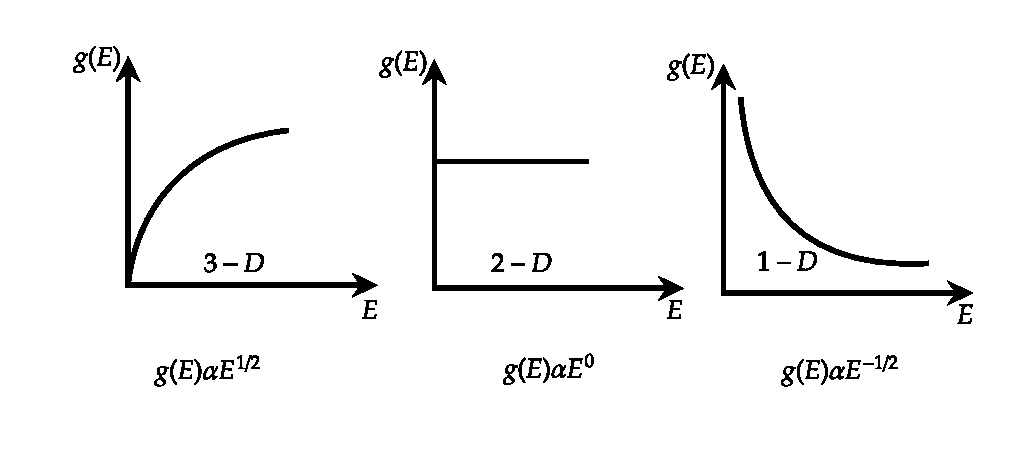
\includegraphics[height=5.5cm,width=13cm]{SP-13}
\end{figure}
\begin{exercise}
	In a classical microcanonical ensemble for a system of $N$ non-interacting particles, the fundamental volume of phase space which is regarded as "equivalent to one-microstate" is 
\end{exercise}
 \begin{tasks}(4)
	\task[\textbf{a.}] $h^{3 N}$
	\task[\textbf{b.}]$h^{2 N}$
	\task[\textbf{c.}]$h^{N}$
	\task[\textbf{d.}]$h$
\end{tasks}
\begin{answer}
	\begin{align*}
	\text{For $N$ non-interacting particles }\text { DOF }&=3 N=f\\
	\text{volume of phase space }&=h^{f}\\
	&=R^{3 N}
	\end{align*}
	So the correct answer is \textbf{Option (a)}
\end{answer}
\textbf{Extremely Relativistic Free Particle: }(E=pc)\\
\renewcommand*{\arraystretch}{1.8}
\begin{tabular}{|p{4cm}|p{4cm}|p{4cm}|}
	\hline
	3-Dimensions & 2-Dimensions & 1-Dimensions\\\hline
	$\Omega(p)=\frac{v \cdot \frac{4}{3} \pi p^{3}}{h^{3}}$&$\Omega(p)=\frac{\pi A p^{2}}{h^{2}}$&$\Omega(p)=\frac{L \times 2 p}{h}$\\
	$\Omega^{\prime}(p)=\frac{4 \pi V p^{2} d p}{h^{3}}$&$\Omega^{\prime}(p)=\frac{2 \pi A p d p}{h^{2}}$&$\Omega^{\prime}(p)=\frac{2 L d p}{h}$\\\hline
	$\Omega(E)=\frac{4 \pi V E^{3}}{3 c^{3} h^{3}}$&$\Omega(E)=\frac{A \pi E^{2}}{C^{2} n^{2}}$&$\Omega(E)=\frac{2 L E}{\hbar c}$\\
	$\Omega(E)=2 \times \frac{4 \pi v\left(E^{2}\right)}{c^{3} h^{3}} d E$&$\Omega^{\prime}(E)=\frac{2 \pi A E}{C^{2} h^{2}}$&$\Omega^{\prime}(E)=\frac{2 L}{R C} d E$\\\hline
\end{tabular}\\\\
Q. Find density of states at energy $E$ of the quantized radiation (photon) is:
 \begin{tasks}(4)
	\task[\textbf{a.}]$\frac{8 \pi v}{h^{3} c^{3}} E^{2}$
	\task[\textbf{b.}]$\frac{8 \pi V}{h^{3} c^{3}} E^{3 / 2}$
	\task[\textbf{c.}]$\frac{8 \pi V}{h^{3} c^{3}} E$
	\task[\textbf{d.}] $\frac{8 \pi V}{h^{3} c^{3}} E^{3 / 2}$
\end{tasks}
\begin{answer}
	\begin{align*}
	\Omega(p)&=\frac{V \times \frac{4}{3} \pi p^{3}}{h^{3}} \Rightarrow \Omega(E)=\frac{4 \pi V E^{3}}{3 c^{3} h^{3}}\\
	\Omega^{\prime}(E)&=\left(\frac{4 \pi V E^{2}}{c^{3} h^{3}} d E\right) \times 2\\
	\Omega^{\prime}(E)&=g(E) d E\\
	g(E)&=\frac{8 \pi V}{c^{3} h^{3}} E^{2}
	\end{align*}
	So the correct answer is \textbf{Option (a)}
\end{answer}
Q. \textbf{For free particle (with $E=ap^s$) with d-DOF: }\\
\begin{align*}
\text{Volume of sphere of radius (R) }V_{d}&=\frac{\pi^{d / 2} R^{d}}{\left(\frac{d}{2}\right) !}\\
\text{area of sphere of radius (R) }s_{d}&=\frac{2 \pi^{d / 2} R^{d-1}}{\left(\frac{d}{2}-1\right) !}\\
\text{ volume of single phase cell }d \tau&=h^{d}\\
g(E)&=\frac{g i V_{d} \pi^{d / 2}\left(\frac{1}{a}\right)^{d / s}\left(\frac{d}{s}\right) E^{(d / s-1)}}{R^{d}(d / 2) !}\\
&g(E) \propto E^{(d / s-1)}\hspace{2cm}d=DOF\\
s&=1 \text{(marsless)},\quad
2 \text{(massive)}
\end{align*}
\begin{exercise}
	For an energy state $E$ of a photon gas, the density of states is proportional to 
\end{exercise}
 \begin{tasks}(4)
	\task[\textbf{a.}] $\sqrt{E}$
	\task[\textbf{b.}] $E $
	\task[\textbf{c.}]$E^{3 / 2}$
	\task[\textbf{d.}] $E^{2}$
\end{tasks}
\begin{answer}
	\begin{align*}
	D(E) &\propto E^{\left(\frac{d}{s}-1\right)}\\
	\text { For proton: } d&=3 \text { and } s=1\\
	D(E) \propto E^{3-1} &\Rightarrow D(E) \alpha E^{2}
	\end{align*}
		So the correct answer is \textbf{Option (d)}
\end{answer}
\begin{exercise}
 The number of states for a system of $N$ indentical free particles in a three dimensional space having total energy between $E$ and $E+\delta E(\delta E<<E),$ is proportional to 
\end{exercise}
 \begin{tasks}(4)
	\task[\textbf{a.}]$E^{\left(\frac{3 N}{2}-1\right)} \delta E$
	\task[\textbf{b.}]$E^{\frac{N}{2}} \delta E$
	\task[\textbf{c.}]$N E^{\frac{1}{2}} \delta E$
	\task[\textbf{d.}]$N^{N} \delta E$ 
\end{tasks}
\begin{answer}
	\begin{align*}
	D(E) &\propto E^{(d / s-1)}\\
	\text { Here } d&=3 \mathrm{~N} \text { and } s=2 \text { (massive) }\\
	D(E) &\propto E^{\left(\frac{3 N}{2}-1\right)}
	\end{align*}
		So the correct answer is \textbf{Option (a)}
\end{answer}
\begin{exercise}
 Draw phase space trajectory of linear (1-dimension) Harmonic oscillator and calculate number of microstate if particle has:\\
	a). sharp value of energy\\
	b). Energy lies between $E$ to $E+d E$
\end{exercise}
\begin{answer}
	\begin{align*}
	E&=\frac{p^{2}}{2 m}+\frac{1}{2} m \omega^2 x^{2}\\
	1&=\frac{p^{2}}{\sqrt{2 m E}}+\frac{x^{2}}{\left(\sqrt{\frac{2 E}{m \omega^2}}\right)^{2}}\\
	\text{area of ellipse }&=\pi a b\\
	\text{volume of single phase cell }&(1-D)=h\\
	\Omega(E)=\frac{\pi a b}{h}&=\frac{\pi \times \sqrt{\frac{2 E}{m \omega^2}}  \times \sqrt{2 m E}}{h}\\
	\Omega(E)&=\frac{2 \pi E}{h \omega}=\frac{E}{h \omega}\\
	\Omega^{\prime}(E)&=\frac{d E}{\hbar \omega}
	\end{align*}
\end{answer}
\begin{note}
	\begin{align*}
	\text{	maxinum valle of }&x \\
\text{	on }x-\text{axis: }p&=0 \hspace{3cm}x_{0}=\sqrt{\frac{2 E_{0}}{m \omega^{2}}}\\
	E_{0}&=0+\frac{1}{2} m u^{2} x_{0}^{2}\hspace{2cm}x_{0} \alpha \sqrt{E_{0}}\\
	\end{align*}
\end{note}






\newpage
\begin{abox}
	Practise set-1
\end{abox}
\begin{enumerate}
	\item Consider an ideal Bose gas in three dimensions with the energy-momentum relation $\varepsilon \propto p^{s}$ with $s>0$. The range of $s$ for which this system may undergo a Bose-Einstein condensation at a non-zero temperature is
{\exyear{NET/JRF(JUNE-2011)}}
\begin{tasks}(4)
\task[\textbf{A.}] $1<s<3$
\task[\textbf{B.}] $0<s<2$
\task[\textbf{C.}] $0<s<3$
\task[\textbf{D.}] $0<s<\infty$
\end{tasks}

\item The internal energy $E$ of a system is given by $E=\frac{b S^{3}}{V N}$, where $b$ is a constant and other symbols have their usual meaning. The temperature of this system is equal to
{\exyear{NET/JRF(JUNE-2011)}}
\begin{tasks}(4)
\task[\textbf{A.}] $\frac{b S^{2}}{V N}$
\task[\textbf{B.}] $\frac{3 b S^{2}}{V N}$
\task[\textbf{C.}]  $\frac{b S^{3}}{V^{2} N}$
\task[\textbf{D.}] $\left(\frac{S}{N}\right)^{2}$
\end{tasks}

\item Consider a Maxwellian distribution of the velocity of the molecules of an ideal gas. Let $V_{m p}$ and $V_{r m s}$ denote the most probable velocity and the root mean square velocity, respectively. The magnitude of the ratio $V_{m p} / V_{r m s}$ is
{\exyear{NET/JRF(DEC-2011)}}
\begin{tasks}(4)
\task[\textbf{A.}] (a) 1
\task[\textbf{B.}] $2 / 3$
\task[\textbf{C.}] $\sqrt{2 / 3}$
\task[\textbf{D.}] $3 / 2$
\end{tasks}

\item If the number density of a free electron gas in three dimensions is increased eight times, its Fermi temperature will
{\exyear{NET/JRF(DEC-2011)}}
\begin{tasks}(2)
\task[\textbf{A.}] Increase by a factor of 4
\task[\textbf{B.}] Decrease by a factor of 4
\task[\textbf{C.}] Increase by a factor of 8
\task[\textbf{D.}] Decrease by a factor of 8
\end{tasks}

\item A one-dimensional chain consists of a set of $N$ rods each of length $a$. When stretched by a load, each rod can align either parallel or perpendicular to the length of the chain. The energy of a rod is $-\varepsilon$ when perpendicular to it. When the chain is in thermal equilibrium at temperature $T$, its average length is
{\exyear{NET/JRF(DEC-2011)}}
\begin{tasks}(2)
\task[\textbf{A.}] $\mathrm{Na} / 2$
\task[\textbf{B.}] $\mathrm{Na}$
\task[\textbf{C.}] $N a /\left(1+e^{-2 \varepsilon / k_{B} T}\right)$
\task[\textbf{D.}] $N a\left(1+e^{-2 \varepsilon / k_{B} T}\right)$
\end{tasks}

\item The excitations of a three-dimensional solid are bosonic in nature with their frequency $\omega$ and wave-number $k$ are related by $\omega \propto k^{2}$ in the large wavelength limit. If the chemical potential is zero, the behavior of the specific heat of the system at low temperature is proportional to
{\exyear{NET/JRF(DEC-2011)}}
\begin{tasks}(4)
\task[\textbf{A.}] $T^{1 / 2}$
\task[\textbf{B.}] $T$
\task[\textbf{C.}]  $T^{3 / 2}$
\task[\textbf{D.}] $T^{3}$
\end{tasks}

\item Gas molecules of mass $m$ are confined in a cylinder of radius $R$ and height $L$ (with $R>>L$ ) kept vertically in the Earth's gravitational field. The average energy of the gas at low temperatures (such that $m g L>>k_{B} T$ ) is given by
{\exyear{NET/JRF(DEC-2011)}}

\begin{tasks}(4)
\task[\textbf{A.}] (a) $N k_{B} T / 2$
\task[\textbf{B.}] $3 N k_{B} T / 2$
\task[\textbf{C.}] $2 N k_{B} T$
\task[\textbf{D.}] $5 N k_{B} T / 2$
\end{tasks}

\item Consider a system of non-interacting particles in $d$ dimensional obeying the dispersion relation $\varepsilon=A k^{s}$, where $\varepsilon$ is the energy, $k$ is the wave vector; $s$ is an integer and $A$ is constant. The density of states, $N(\varepsilon)$, is proportional to
{\exyear{NET/JRF(JUNE-2012)}}

\begin{tasks}(4)
\task[\textbf{A.}] $\varepsilon^{\frac{s}{d}-1}$
\task[\textbf{B.}] $\varepsilon^{\frac{d}{s}-1}$
\task[\textbf{C.}] $\varepsilon^{\frac{d}{s}+1}$
\task[\textbf{D.}] $\varepsilon^{\frac{s}{d}+1}$
\end{tasks}


\item The number of ways in which $\mathrm{N}$ identical bosons can be distributed in two energy levels, is
{\exyear{NET/JRF(JUNE-2012)}}
\begin{tasks}(4)
\task[\textbf{A.}] $N+1$
\task[\textbf{B.}] $\frac{N(N-1)}{2}$
\task[\textbf{C.}] $\frac{N(N+1)}{2}$
\task[\textbf{D.}] $N$
\end{tasks}

\item The free energy of the gas of $N$ particles in a volume $V$ and at a temperature $T$ is $F=N k_{B} T \ln \left[a_{0} V\left(k_{B} T\right)^{5 / 2} / N\right]$, where $a_{0}$ is a constant and $k_{B}$ denotes the Boltzmann constant. The internal energy of the gas is
{\exyear{NET/JRF(JUNE-2012)}}

\begin{tasks}(2)
\task[\textbf{A.}] $\frac{3}{2} N k_{B} T$
\task[\textbf{B.}] $\frac{5}{2} N k_{B} T$
\task[\textbf{C.}] $N k_{B} T \ln \left[a_{0} V\left(k_{B} T\right)^{5 / 2} / N\right]-\frac{3}{2} N k_{B} T$
\task[\textbf{D.}] $N k_{B} T \ln \left[a_{0} V /\left(k_{B} T\right)^{5 / 2}\right]$
\end{tasks}


\item A system has two normal modes of vibration, with frequencies $\omega_{1}$ and $\omega_{2}=2 \omega_{1} .$ What is the probability that at temperature $T$, the system has an energy less than $4 \hbar \omega_{1}$ ?
[In the following $x=e^{-\beta \hbar \omega_{1}}$ and $Z$ is the partition function of the system.]
{\exyear{NET/JRF(JUNE-2012)}}

\begin{tasks}(2)
\task[\textbf{A.}] $x^{3 / 2}\left(x+2 x^{2}\right) / Z$
\task[\textbf{B.}] $x^{3 / 2}\left(1+x+x^{2}\right) / Z$
\task[\textbf{C.}] $x^{3 / 2}\left(1+2 x^{2}\right) / Z$
\task[\textbf{D.}]  $x^{3 / 2}\left(1+x+2 x^{2}\right) / Z$
\end{tasks}


\item Bose condensation occurs in liquid $H e^{4}$ kept at ambient pressure at $2.17 K$. At which temperature will Bose condensation occur in $H e^{4}$ in gaseous state, the density of which is 1000 times smaller than that of liquid $H e^{4}$ ? (Assume that it is a perfect Bose gas.)
{\exyear{NET/JRF(JUNE-2012)}}

\begin{tasks}(4)
\task[\textbf{A.}] $2.17 \mathrm{mK}$
\task[\textbf{B.}] $21.7 \mathrm{mK}$
\task[\textbf{C.}] $21.7 \mu K$
\task[\textbf{D.}] $2.17 \mu K$
\end{tasks}

\item Consider black body radiation contained in a cavity whose walls are at temperature $T$. The radiation is in equilibrium with the walls of the cavity. If the temperature of the walls is increased to $2 T$ and the radiation is allowed to come to equilibrium at the new temperature, the entropy of the radiation increases by a factor of
{\exyear{NET/JRF(JUNE-2012)}}

\begin{tasks}(4)
\task[\textbf{A.}] 2
\task[\textbf{B.}] 4
\task[\textbf{C.}] 8
\task[\textbf{D.}] 16
\end{tasks}

\item Consider a one-dimensional Ising model with $N$ spins, at very low temperatures when almost all spins are aligned parallel to each other. There will be a few spin flips with each flip costing an energy $2 J .$ In a configuration with $r$ spin flips, the energy of the system is $E=-N J+2 r J$ and the number of configuration is ${ }^{N} C_{r} ; r$ varies from 0 to $N$. The partition function is
{\exyear{NET/JRF(DEC-2012)}}

\begin{tasks}(4)
\task[\textbf{A.}] $\left(\frac{J}{k_{B} T}\right)^{N}$
\task[\textbf{B.}]  $e^{-N J / k_{B} T}$
\task[\textbf{C.}] $\left(\sinh \frac{J}{k_{B} T}\right)^{N}$
\task[\textbf{D.}] $\left(\cosh \frac{J}{k_{B} T}\right)^{N}$
\end{tasks}


\item Consider a system of three spins $S_{1}, S_{2}$ and $S_{3}$ each of which can take values $+1$ and $-1 .$ The energy of the system is given by $E=-J\left[S_{1} S_{2}+S_{2} S_{3}+S_{3} S_{1}\right]$ where $J$ is a positive constant. The minimum energy and the corresponding number of spin configuration are, respectively,
{\exyear{NET/JRF(DEC-2012)}}

\begin{tasks}(4)
\task[\textbf{A.}] $J$ and 1
\task[\textbf{B.}] $-3 J$ and 1
\task[\textbf{C.}] $-3 J$ and 2
\task[\textbf{D.}] $-6 J$ and 2
\end{tasks}
\newcommand*{\downuparrow}[1]{\ensuremath{\overset{\uparrow}{#1}}}
\newcommand*{\downdownarrow}[1]{\ensuremath{\overset{\downarrow}{#1}}}


	\item A system of non-interacting spin-1/2 charged particles are placed in an extemal magnetic field. At low temperature $T$, the leading behavior of the excess energy above the ground state energy, depends on $T$ as: $(c$ is a constant)
	{\exyear{NET/JRF(JUNE-2013)}}

\begin{tasks}(2)
	\task[\textbf{A.}] $c T$
	\task[\textbf{B.}]  $c T^{3}$
	\task[\textbf{C.}] $e^{-c / T}$
	\task[\textbf{D.}] $c$ (is independent of $T$ )
\end{tasks}


	\item Consider a system of two Ising spins $S_{1}$ and $S_{2}$ taking values $\pm 1$ with interaction energy given by $\varepsilon=-J S_{1} S_{2}$, when it is in thermal equilibrium at temperature $T$. For large $T$, the average energy of the system varies as $C / k_{B} T$, with $C$ given by
	{\exyear{NET/JRF(JUNE-2013)}}

\begin{tasks}(4)
	\task[\textbf{A.}]  $-2 J^{2}$
	\task[\textbf{B.}] $-J^{2}$
	\task[\textbf{C.}] $J^{2}$
	\task[\textbf{D.}] $4 J$
\end{tasks}


	\item Consider two different systems each with three identical non-interacting particles. Both have single particle states with energies $\varepsilon_{0}, 3 \varepsilon_{0}$ and $5 \varepsilon_{0},\left(\varepsilon_{0}>0\right)$. One system is populated by spin $-\frac{1}{2}$ fermions and the other by bosons. What is the value of $E_{F}-E_{B}$ where $E_{F}$ and $E_{B}$ are the ground state energies of the fermionic and bosonic systems respectively?
    	{\exyear{NET/JRF(JUNE-2013)}}

\begin{tasks}(4)
	\task[\textbf{A.}] $6 \varepsilon_{0}$
	\task[\textbf{B.}] $2 \varepsilon_{0}$
	\task[\textbf{C.}] $4 \varepsilon_{0}$.
	\task[\textbf{D.}] $\varepsilon_{0}$
\end{tasks}


	\item Three identical spin- $\frac{1}{2}$ fermions are to be distributed in two non-degenerate distinct energy levels. The number of ways this can be done is
	{\exyear{NET/JRF(DEC-2013)}}

\begin{tasks}(4)
	\task[\textbf{A.}] 8
	\task[\textbf{B.}] 4
	\task[\textbf{C.}] 3
	\task[\textbf{D.}] 2
\end{tasks}


	\item Which of the graphs below gives the correct qualitative behaviour of the energy density $E_{r}(\lambda)$ of blackbody radiation of wavelength $\lambda$ at two temperatures $T_{1}$ and $T_{2}\left(T_{1}<T_{2}\right) ?$
	{\exyear{NET/JRF(JUNE-2014)}}

\begin{tasks}(2)
	\task[\textbf{A.}] \begin{figure}[H]
		\centering
		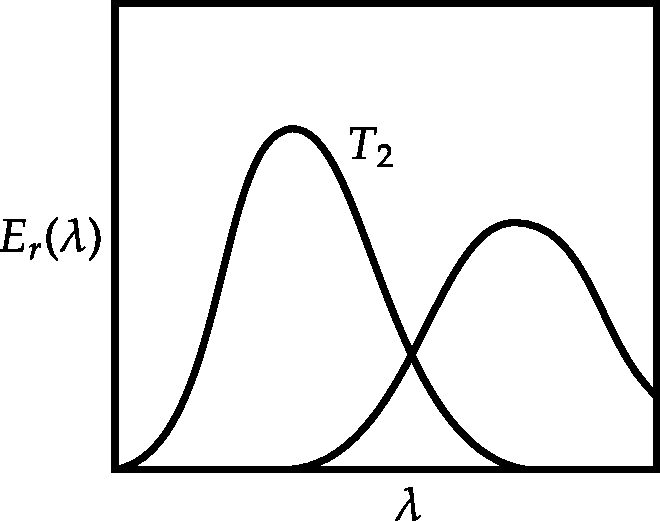
\includegraphics[height=4cm,width=5cm]{diagram-20210924(10)-crop}
	\end{figure}
	\task[\textbf{B.}] \begin{figure}[H]
		\centering
		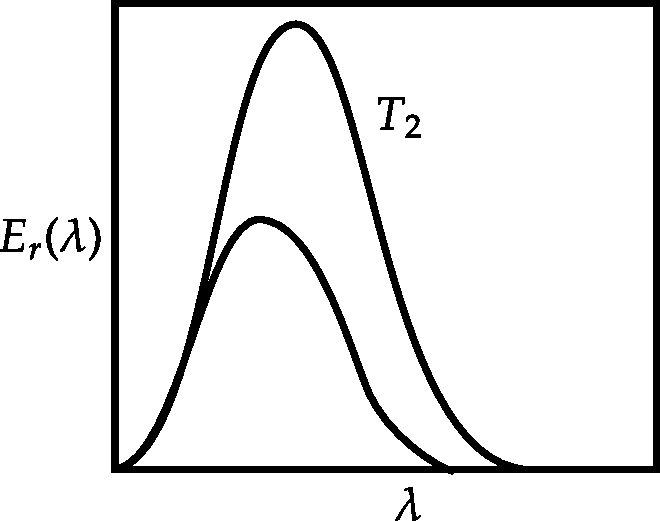
\includegraphics[height=4cm,width=5cm]{diagram-20210924(11)-crop}
	\end{figure}
	\task[\textbf{C.}] \begin{figure}[H]
		\centering
		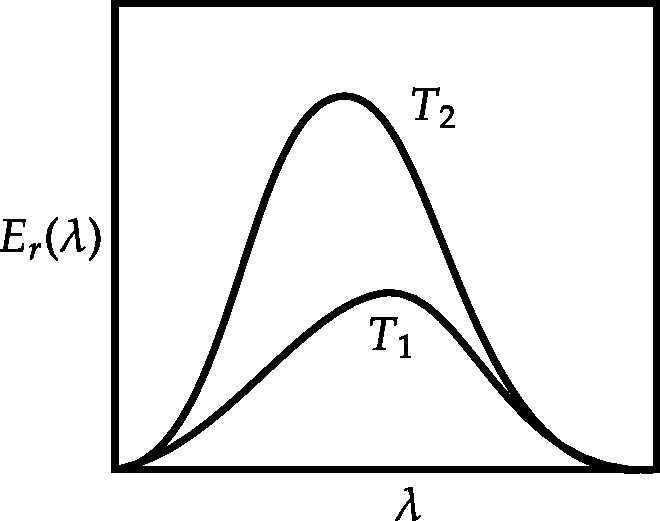
\includegraphics[height=4cm,width=5cm]{diagram-20210924(12)-crop}
	\end{figure}
	\task[\textbf{D.}] \begin{figure}[H]
		\centering
		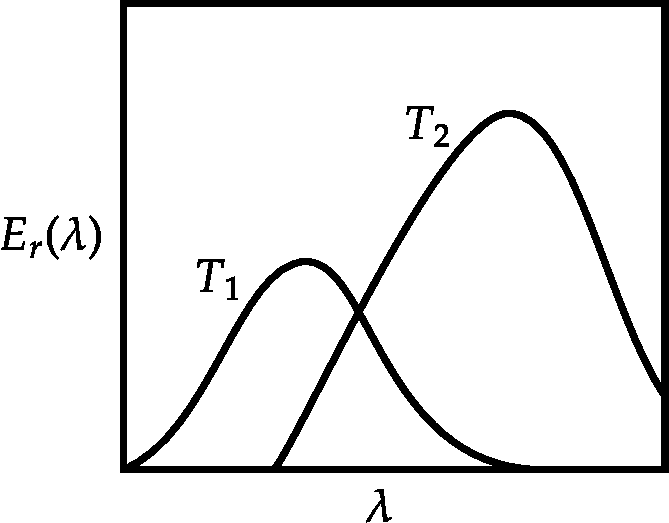
\includegraphics[height=4cm,width=5cm]{diagram-20210924(13)-crop}
	\end{figure}
\end{tasks}

	\item The pressure of a non-relativistic free Fermi gas in three-dimensions depends, at $T=0$, on the density of fermions $n$ as
	{\exyear{NET/JRF(JUNE-2014)}}
\begin{tasks}(4)
	\task[\textbf{A.}] $n^{5 / 3}$
	\task[\textbf{B.}] $n^{1 / 3}$
	\task[\textbf{C.}]  $n^{2 / 3}$
	\task[\textbf{D.}] $n^{4 / 3}$
\end{tasks}

	\item A collection $N$ of non-interacting spins $S_{i}, i=1,2, \ldots ., N,\left(S_{i}=\pm 1\right)$ is kept in an external magnetic field $B$ at a temperature $T .$ The Hamiltonian of the system is $H=-\mu B \Sigma_{i} S_{i} .$ What should be the minimum value of $\frac{\mu B}{k_{B} T}$ for which the mean value $\left\langle S_{i}\right\rangle \geq \frac{1}{3} ?$
	{\exyear{NET/JRF(DEC-2014)}}
\begin{tasks}(4)
	\task[\textbf{A.}]  $\frac{1}{2} N \ln 2$
	\task[\textbf{B.}] $2 \ln 2$
	\task[\textbf{C.}] $\frac{1}{2} \ln 2$
	\task[\textbf{D.}]  $N \ln 2$
\end{tasks}

	\item Consider three Ising spins at the vertices of a triangle which interact with each other with a ferromagnetic Ising interaction of strength $J .$ The partition function of the system at temperature $T$ is given by $\left(\beta=\frac{1}{k_{B} T}\right):$
	{\exyear{NET/JRF(JUNE-2015)}}

\begin{tasks}(2)
	\task[\textbf{A.}]  $2 e^{3 \beta J}+6 e^{-\beta J}$
	\task[\textbf{B.}] $2 e^{-3 \beta J}+6 e^{\beta J}$
	\task[\textbf{C.}] $2 e^{3 \beta J}+6 e^{-3 \beta J}+3 e^{\beta J}+3 e^{-\beta J}$
	\task[\textbf{D.}] $(2 \cosh \beta J)^{3}$
\end{tasks}


	\item An ideal Bose gas in $d$-dimensions obeys the dispersion relation $\in(\vec{k})=A k^{s}$, where $A$ and $s$ are constants. For Bose-Einstein condensation to occur, the occupancy of excited states
	$$
	N_{e}=c \int_{0}^{\infty} \frac{\epsilon^{\frac{(d-s)}{s}}}{\left(e^{\beta(\epsilon-\mu)}-1\right)} d \in
	$$
	where $c$ is a constant, should remain finite even for $\mu=0$. This can happen if
	{\exyear{NET/JRF(JUNE-2015)}}

\begin{tasks}(4)
	\task[\textbf{A.}] $\frac{d}{s}<\frac{1}{4}$
	\task[\textbf{B.}] $\frac{1}{4}<\frac{d}{s}<\frac{1}{2}$
	\task[\textbf{C.}] $\frac{d}{s}>1$
	\task[\textbf{D.}] $\frac{1}{2}<\frac{d}{s}<1$
\end{tasks}

	\item For a system of independent non interacting one-dimensional oscillators, the value of the free energy per oscillator, in the limit $T \rightarrow 0$, is
	{\exyear{NET/JRF(DEC-2015)}}
\begin{tasks}(4)
	\task[\textbf{A.}] $\frac{1}{2} \hbar \omega$
	\task[\textbf{B.}] $\hbar \omega$
	\task[\textbf{C.}] $\frac{3}{2} \hbar \omega$
	\task[\textbf{D.}] 0
\end{tasks}

\end{enumerate}
\colorlet{ocre1}{ocre!70!}
\colorlet{ocrel}{ocre!30!}
\setlength\arrayrulewidth{1pt}
\begin{table}[H]
	\centering
	\arrayrulecolor{ocre}
	\begin{tabular}{|p{1.5cm}|p{1.5cm}||p{1.5cm}|p{1.5cm}|}
		\hline
		\multicolumn{4}{|c|}{\textbf{Answer key}}\\\hline\hline
		\rowcolor{ocrel}Q.No.&Answer&Q.No.&Answer\\\hline
		1&\textbf{A} &2&\textbf{B}\\\hline
		3&\textbf{C} &4&\textbf{A} \\\hline
		5&\textbf{C} &6&\textbf{C} \\\hline
		7&\textbf{D}&8&\textbf{B}\\\hline
		9&\textbf{A}&10&\textbf{B}\\\hline
		11&\textbf{D} &12&\textbf{B}\\\hline
		13&\textbf{C}&14&\textbf{D}\\\hline
		15&\textbf{C}&16 &\textbf{C}\\\hline
		17&\textbf{B}&18 &\textbf{B}\\\hline
		19&\textbf{B}&20 &\textbf{C}\\\hline
		21&\textbf{A}&22 &\textbf{C}\\\hline
		23&\textbf{B}&24 &\textbf{C}\\\hline
		25 &\textbf{A}& &\\\hline
	\end{tabular}
\end{table}
\begin{abox}
	Practise set-2
\end{abox}
\begin{enumerate}
	\item Consider a system of two particles $A$ and $B$. Each particle can occupy one of three possible quantum states $|1\rangle,|2\rangle$ and $|3\rangle$. The ratio of the probability that the two particles
	are in the same state to the probability that the two particles are in different states is calculated for bosons and classical (Maxwell-Boltzmann) particles. They are respectively
	{\exyear{JEST 2013}}
	
	\begin{tasks}(4)
		\task[\textbf{A.}] 1,0
		\task[\textbf{B.}]  $\frac{1}{2}, 1$
		\task[\textbf{C.}] $1, \frac{1}{2}$
		\task[\textbf{D.}] $0, \frac{1}{2}$
	\end{tasks}
	
	\item Consider three situations of 4 particles in one dimensional box of width $L$ with hard walls. In case (i), the particles are fermions, in case (ii) they are bosons, and in case (iii) they are classical. If the total ground state energy of the four particles in these three cases are $E_{F}, E_{B}$ and $E_{c l}$ respectively, which of the following is true?
	{\exyear{JEST 2013}}
		\begin{tasks}(2)
		\task[\textbf{A.}] $E_{F}=E_{B}=E_{c l}$
		\task[\textbf{B.}] $E_{F}>E_{B}=E_{c l}$
		\task[\textbf{C.}] $E_{F}<E_{B}<E_{c l}$
		\task[\textbf{D.}] $E_{F}>E_{B}>E_{c l}$
	\end{tasks}

	\item If the mean square fluctuations in energy of a system in equilibrium at temperature $T$ is proportional to $T^{\alpha}$, then the energy of the system is proportional to
	{\exyear{JEST 2017}}
	\begin{tasks}(4)
		\task[\textbf{A.}] $T^{\alpha-2}$
		\task[\textbf{B.}] $T^{\frac{\alpha}{2}}$
		\task[\textbf{C.}] $T^{\alpha-1}$
		\task[\textbf{D.}] $T^{\alpha}$
	\end{tasks}
	\item For a two-dimensional free electron gas, the electronic density $\mathrm{n}$, and the Fermi energy $\mathrm{E}_{\mathrm{F}}$, are related by
	{\exyear{GATE 2010}}
	\begin{tasks}(4)
		\task[\textbf{A.}] $n=\frac{\left(2 m E_{F}\right)^{3 / 2}}{3 \pi^{2} \hbar^{3}}$
		\task[\textbf{B.}] $n=\frac{m E_{F}}{\pi \hbar^{2}}$
		\task[\textbf{C.}] $n=\frac{m E_{F}}{2 \pi \hbar^{2}}$
		\task[\textbf{D.}] $n=\frac{\left(2 m E_{F}\right)^{3 / 2}}{\pi \hbar}$
	\end{tasks}
	
	\item For an ideal Fermi gas in three dimensions, the electron velocity $V_{F}$ at the Fermi surface is related to electron concentration $n$ as,
	{\exyear{GATE 2012}}
	
	\begin{tasks}(4)
		\task[\textbf{A.}] $V_{F} \propto n^{2 / 3}$
		\task[\textbf{B.}]  $V_{F} \propto n$
		\task[\textbf{C.}] $V_{F} \propto n^{1 / 2}$
		\task[\textbf{D.}] $V_{F} \propto n^{1 / 3}$
	\end{tasks}
	
	\item The total energy, $E$ of an ideal non-relativistic Fermi gas in three dimensions is given by $E \propto \frac{N^{5 / 3}}{V^{2 / 3}}$, where $N$ is the number of particles and $V$ is the volume of the gas. Identify the CORRECT equation of state ( $P$ being the pressure),
	{\exyear{GATE 2012}}
	\begin{tasks}(4)
		\task[\textbf{A.}] $P V=\frac{1}{3} E$
		\task[\textbf{B.}] $P V=\frac{2}{3} E$
		\task[\textbf{C.}] $P V=E$
		\task[\textbf{D.}] $P V=\frac{5}{3} E$
	\end{tasks}
	
	\item Consider a linear collection of $N$ independent spin $1 / 2$ particles, each at a fixed location. The entropy of this system is $(k$ is the Boltzmann constant)
	{\exyear{GATE 2013}}
	\begin{tasks}(4)
		\task[\textbf{A.}] Zero
		\task[\textbf{B.}]  $N k$
		\task[\textbf{C.}]  $\frac{1}{2} N k$
		\task[\textbf{D.}] $N k \ln (2)$
	\end{tasks}
	
	\item Two identical fermions
	{\exyear{GATE 2013}}
	\begin{tasks}(2)
		\task[\textbf{A.}] $e^{-2 \beta E}+e^{-4 \beta E}+e^{-6 \beta E}+e^{-8 \beta E}$
		\task[\textbf{B.}] $e^{-3 \beta E}+e^{-4 \beta E}+e^{-5 \beta E}+e^{-6 \beta E}+e^{-7 \beta E}$
		\task[\textbf{C.}] $\left(e^{-\beta E}+e^{-2 \beta E}+e^{-3 \beta E}+e^{-4 \beta E}\right)^{2}$
		\task[\textbf{D.}] $e^{-2 \beta E}-e^{-4 \beta E}+e^{-6 \beta E}-e^{-8 \beta E}$
	\end{tasks}

	\begin{minipage}{\textwidth}
		\item Two distinguishable particles
		{\exyear{GATE 2014}}
	\end{minipage}
	\begin{tasks}(2)
		\task[\textbf{A.}] $e^{-2 \beta E}+e^{-4 \beta E}+e^{-6 \beta E}+e^{-8 \beta E}$
		\task[\textbf{B.}] $e^{-3 \beta E}+e^{-4 \beta E}+e^{-5 \beta E}+e^{-6 \beta E}+e^{-7 \beta E}$
		\task[\textbf{C.}] $\left(e^{-\beta E}+e^{-2 \beta E}+e^{-3 \beta E}+e^{-4 \beta E}\right)^{2}$
		\task[\textbf{D.}] $e^{-2 \beta E}-e^{-4 \beta E}+e^{-6 \beta E}-e^{-8 \beta E}$
	\end{tasks}

	\item For a system of two bosons each of which can occupy any of the two energy levels 0 and $\varepsilon$. The mean energy of the system at temperature $T$ with $\beta=\frac{1}{k_{\beta} T}$ is given by
	{\exyear{GATE 2014}}
	
	\begin{tasks}(4)
		\task[\textbf{A.}] $\frac{\varepsilon e^{-\beta \varepsilon}+2 \varepsilon e^{-2 \beta \varepsilon}}{1+2 e^{-\beta \varepsilon}+e^{-2 \beta \varepsilon}}$
		\task[\textbf{B.}] $\frac{1+\varepsilon e^{-\beta \varepsilon}}{2 e^{-\beta \varepsilon}+e^{-2 \beta \varepsilon}}$
		\task[\textbf{C.}] $\frac{2 \varepsilon e^{-\beta \varepsilon}+\varepsilon e^{-2 \beta \varepsilon}}{2+e^{-\beta \varepsilon}+e^{-2 \beta \varepsilon}}$
		\task[\textbf{D.}] $\frac{\varepsilon e^{-\beta \varepsilon}+2 \varepsilon e^{-2 \beta \varepsilon}}{2+e^{-\beta \varepsilon}+e^{-2 \beta \varepsilon}}$
	\end{tasks}

	\begin{minipage}{\textwidth}
		\item Consider a system of 3 fermions which can occupy any of the 4 available energy states with equal probability. The entropy of the system is
		{\exyear{GATE 2014}}
	\end{minipage}
	\begin{tasks}(4)
		\task[\textbf{A.}] $k_{B} \ln 2$
		\task[\textbf{B.}] $2 k_{B} \ln 2$
		\task[\textbf{C.}]  $2 k_{B} \ln 4$
		\task[\textbf{D.}]  $3 k_{B} \ln 4$
	\end{tasks}
	\item In Boss-Einstein condensation, the particles
	{\exyear{GATE 2015}}
		\begin{tasks}(1)
		\task[\textbf{A.}] Have strong interparticle attraction
		\task[\textbf{B.}] Condense in real space
		\task[\textbf{C.}]  Have overlapping wavefunctions
		\task[\textbf{D.}] Have large and positive chemical potential
	\end{tasks}

	\begin{minipage}{\textwidth}
		\item For a black body radiation in a cavity, photons are created and annihilated freely as a result of emission and absorption by the walls of the cavity. This is because
		{\exyear{GATE 2015}}
	\end{minipage}
	\begin{tasks}(1)
		\task[\textbf{A.}] The chemical potential of the photons is zero
		\task[\textbf{B.}] Photons obey Pauli exclusion principle
		\task[\textbf{C.}] Photons are spin-1 particles
		\task[\textbf{D.}] The entropy of the photons is very large
	\end{tasks}
	
	\item The total power emitted by a spherical black body of radius $R$ at a temperature $T$ is $P_{1}$. Let $P_{2}$ be the total power emitted by another spherical black body of radius $\frac{R}{2}$ kept at temperature $2 T$. The ratio, $\frac{P_{1}}{P_{2}}$ is----------- (Give your answer upto two decimal places)
	{\exyear{GATE 2016}}
	
	
	\item Consider a system having three energy levels with energies $0,2 \varepsilon$ and $3 \varepsilon$, with respective degeneracies of 2,2 and 3 . Four bosons of spin zero have to be accommodated in these levels such that the total energy of the system is $10 \varepsilon$. The number of ways in which it can be done is------------
	{\exyear{GATE 2016}}
	
	\item Consider a triatomic molecule of the shape shown in the figure in three dimensions. The heat capacity of this molecule at high temperature (temperature much higher than the vibrational and rotational energy scales of the molecule but lower than its bond dissociation energies) is:
	{\exyear{GATE 2017}}
	\begin{figure}[H]
		\centering
		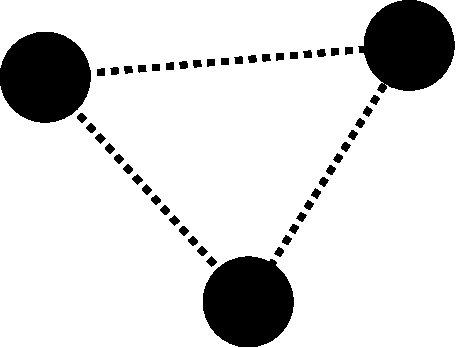
\includegraphics[height=3cm,width=4.5cm]{diagram-20210911(13)-crop}
	\end{figure}
	\begin{tasks}(4)
		\task[\textbf{A.}] $\frac{3}{2} k_{B}$
		\task[\textbf{B.}] $3 k_{B}$
		\task[\textbf{C.}] $\frac{9}{2} k_{B}$
		\task[\textbf{D.}] $6 k_{B}$
	\end{tasks}

	\item Consider two particles and two non-degenerate quantum levels 1 and $2 .$ Level 1 always contains a particle. Hence, what is the probability that level 2 also contains a particle for each of the two cases:\\
	(i) when the two particles are distinguishable and (ii) when the two particles are bosons?
	{\exyear{GATE 2017}}
	\begin{tasks}(2)
		\task[\textbf{A.}] (i) $\frac{1}{2}$ and (ii) $\frac{1}{3}$
		\task[\textbf{B.}] (i) $\frac{1}{2}$ and (ii) $\frac{1}{2}$
		\task[\textbf{C.}] (i) $\frac{2}{3}$ and (ii) $\frac{1}{2}$
		\task[\textbf{D.}] (i) 1 and (ii) 0
	\end{tasks}

\end{enumerate}	
\colorlet{ocre1}{ocre!70!}
\colorlet{ocrel}{ocre!30!}
\setlength\arrayrulewidth{1pt}
\begin{table}[H]
	\centering
	\arrayrulecolor{ocre}
	\begin{tabular}{|p{1.5cm}|p{1.5cm}||p{1.5cm}|p{1.5cm}|}
		\hline
		\multicolumn{4}{|c|}{\textbf{Answer key}}\\\hline\hline
		\rowcolor{ocrel}Q.No.&Answer&Q.No.&Answer\\\hline
		1&\textbf{C} &2&\textbf{B}\\\hline
		3&\textbf{C} &4&\textbf{D} \\\hline
		5&\textbf{D} &6&\textbf{B} \\\hline
		7&\textbf{D}&8&\textbf{B}\\\hline
		9&\textbf{C}&10&\textbf{A}\\\hline
		11&\textbf{B} &12&\textbf{C}\\\hline
		13&\textbf{A}&14&\textbf{0.25}\\\hline
		15&\textbf{18}&16 &\textbf{D}\\\hline
		17&\textbf{C}&\\\hline
		
	\end{tabular}
\end{table}